\section{LEP und der OPAL Detektor}
\subsection{LEP am CERN}
%LEP luftaufnahme
\begin{frame}
	\frametitle{Der LEP Speicherring}
	\begin{figure}[ht]
		\centering
		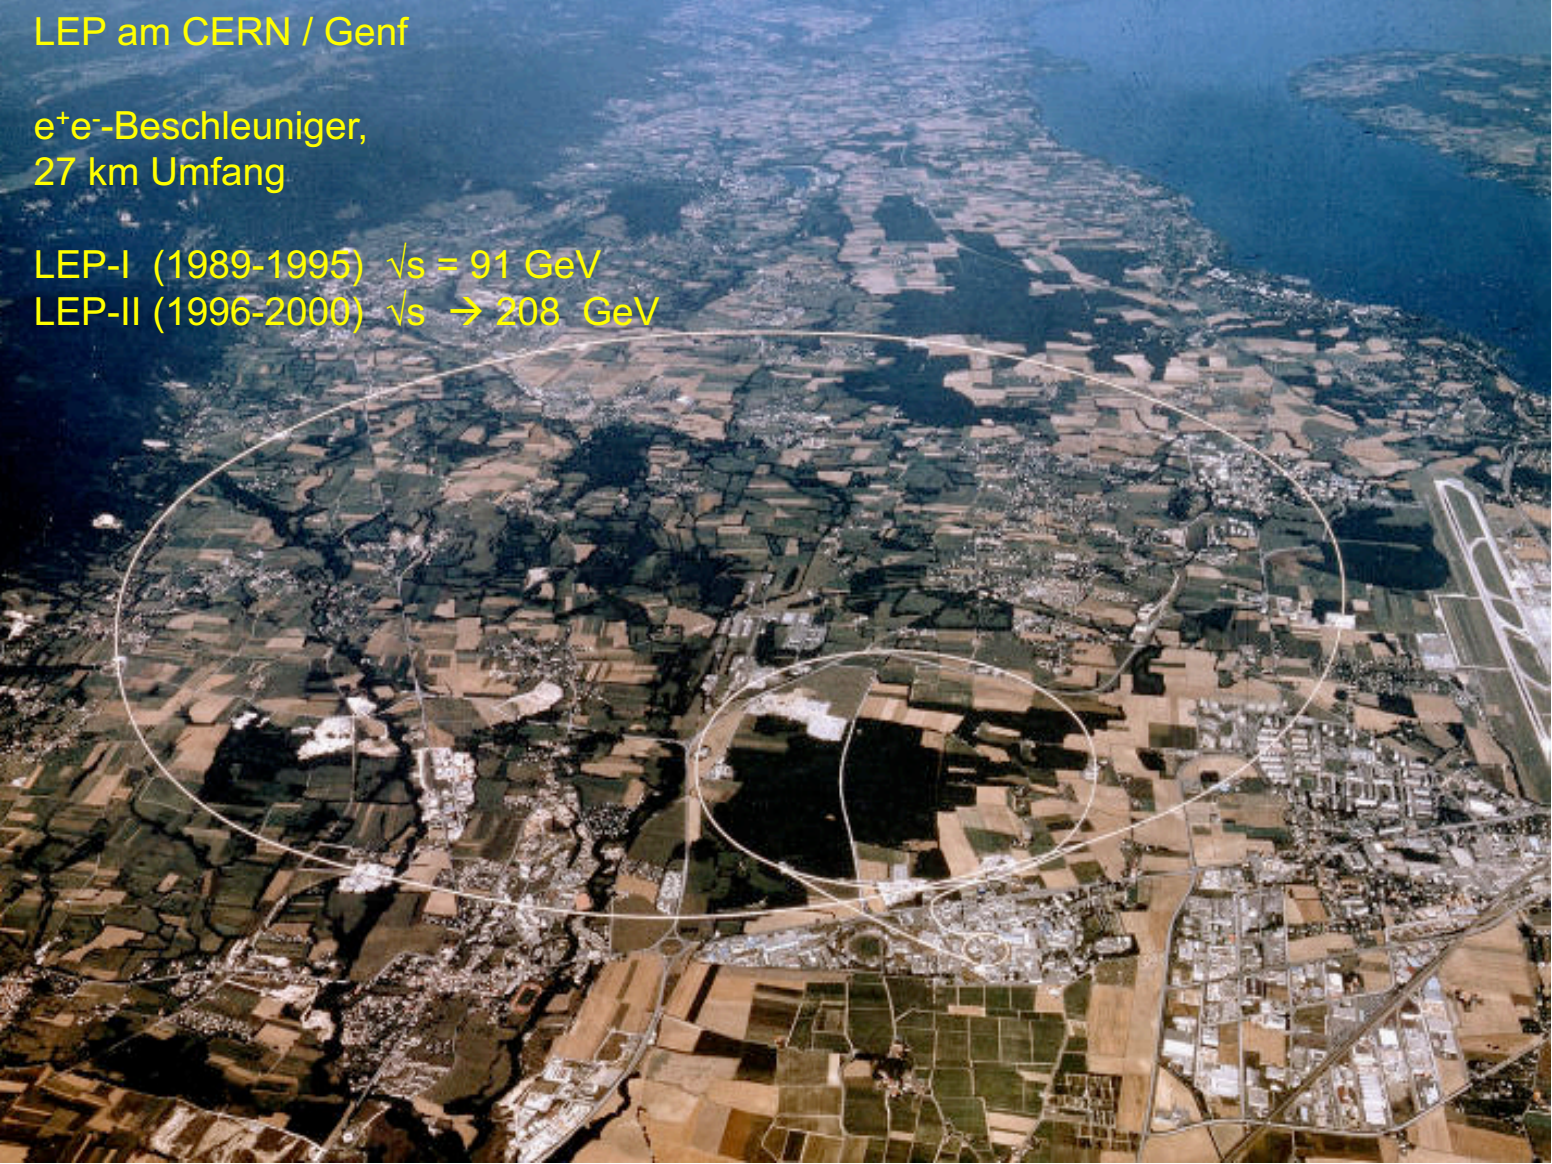
\includegraphics[width=1.0\linewidth]{graphics/LEPmap}
		\caption[Bird's eye view LEP]{Bird's eye view of the Large Electron-Positron Collider at Cern in Geneva, Switzerland. Today the large circular collider tunnel is used for the Large Hadron Collider (LHC)\cite{jakobs}. The smaller circle belonged to the Super Proton Synchroton (SPS) experiment.}
		\label{fig:LEPmap}
	\end{figure}
\end{frame}

\begin{frame}
	\frametitle{Der LEP Speicherring}
	
\end{frame}

\subsection{Der OPAL Detektor}
\begin{frame}
	\frametitle{Schematischer Aufbau}
\end{frame}

\begin{frame}
	\frametitle{Driftkammer}
	
\end{frame}
\begin{frame}
	\frametitle{Elektromagnetisches Kalorimeter}
	
\end{frame}

\begin{frame}
	\frametitle{Hadronisches Kalorimeter}
	
\end{frame}

\begin{frame}
	\frametitle{Myonenkammer}
	
\end{frame}


